\PassOptionsToPackage{unicode=true}{hyperref} % options for packages loaded elsewhere
\PassOptionsToPackage{hyphens}{url}
%
\documentclass[]{article}
\usepackage{lmodern}
\usepackage{amssymb,amsmath}
\usepackage{ifxetex,ifluatex}
\usepackage{fixltx2e} % provides \textsubscript
\ifnum 0\ifxetex 1\fi\ifluatex 1\fi=0 % if pdftex
  \usepackage[T1]{fontenc}
  \usepackage[utf8]{inputenc}
  \usepackage{textcomp} % provides euro and other symbols
\else % if luatex or xelatex
  \usepackage{unicode-math}
  \defaultfontfeatures{Ligatures=TeX,Scale=MatchLowercase}
\fi
% use upquote if available, for straight quotes in verbatim environments
\IfFileExists{upquote.sty}{\usepackage{upquote}}{}
% use microtype if available
\IfFileExists{microtype.sty}{%
\usepackage[]{microtype}
\UseMicrotypeSet[protrusion]{basicmath} % disable protrusion for tt fonts
}{}
\IfFileExists{parskip.sty}{%
\usepackage{parskip}
}{% else
\setlength{\parindent}{0pt}
\setlength{\parskip}{6pt plus 2pt minus 1pt}
}
\usepackage{hyperref}
\hypersetup{
            pdftitle={Effect of mandatory jail sentence on State vehicel fatality rate},
            pdfborder={0 0 0},
            breaklinks=true}
\urlstyle{same}  % don't use monospace font for urls
\usepackage[margin=1in]{geometry}
\usepackage{graphicx,grffile}
\makeatletter
\def\maxwidth{\ifdim\Gin@nat@width>\linewidth\linewidth\else\Gin@nat@width\fi}
\def\maxheight{\ifdim\Gin@nat@height>\textheight\textheight\else\Gin@nat@height\fi}
\makeatother
% Scale images if necessary, so that they will not overflow the page
% margins by default, and it is still possible to overwrite the defaults
% using explicit options in \includegraphics[width, height, ...]{}
\setkeys{Gin}{width=\maxwidth,height=\maxheight,keepaspectratio}
\setlength{\emergencystretch}{3em}  % prevent overfull lines
\providecommand{\tightlist}{%
  \setlength{\itemsep}{0pt}\setlength{\parskip}{0pt}}
\setcounter{secnumdepth}{0}
% Redefines (sub)paragraphs to behave more like sections
\ifx\paragraph\undefined\else
\let\oldparagraph\paragraph
\renewcommand{\paragraph}[1]{\oldparagraph{#1}\mbox{}}
\fi
\ifx\subparagraph\undefined\else
\let\oldsubparagraph\subparagraph
\renewcommand{\subparagraph}[1]{\oldsubparagraph{#1}\mbox{}}
\fi

% set default figure placement to htbp
\makeatletter
\def\fps@figure{htbp}
\makeatother


\title{Effect of mandatory jail sentence on State vehicel fatality rate}
\author{}
\date{\vspace{-2.5em}}

\begin{document}
\maketitle

\begin{center}\rule{0.5\linewidth}{0.5pt}\end{center}

\hypertarget{team-id-team-6}{%
\subsubsection{Team ID: Team 6}\label{team-id-team-6}}

\hypertarget{name-connor-rosenberg}{%
\paragraph{NAME: Connor Rosenberg}\label{name-connor-rosenberg}}

\hypertarget{name-rongkui-han}{%
\paragraph{NAME: Rongkui Han}\label{name-rongkui-han}}

\hypertarget{name-yuqing-yang}{%
\paragraph{NAME: Yuqing Yang}\label{name-yuqing-yang}}

\hypertarget{name-nassim-ali-chaouche}{%
\paragraph{NAME: Nassim Ali-Chaouche}\label{name-nassim-ali-chaouche}}

\begin{center}\rule{0.5\linewidth}{0.5pt}\end{center}

\hypertarget{introduction}{%
\subsection{1.0 Introduction}\label{introduction}}

\hypertarget{background}{%
\paragraph{1.1 Background}\label{background}}

Traffic accidents cause thousands of deaths in the United States every
year. Data pertinent to US traffic fatalities from the years 1982 to
1988 can be easily accessed in the ``Fatalities'' dataset. The data was
obtained from sources such as the US Department of Transportation Fatal
Accident Reporting System (FARS) and the US Bureau of Labor Statistics.
The dataset includes panel data for 48 states (Alaska and Hawaii not
included), containing demographic variables such as population, income
per capita, religious belief, and unemployment rate. In addition,
features that are commonly associated with traffic accidents and its
regulation, such as average miles per driver, percentage of young
drivers, tax collected per case of beer, presence of a preliminary
breath test law, and whether the state implemented mandatory jail
sentences or community service for an initial drunk driving conviction,
were also presented in the dataset. Finally, the number of vehicle
fatalities and its numerous subsets, such as night-time or
single-vehicle fatalities, were introduced. The observations were
recorded for each state annually. In total, there are 336 observations
recorded for 34 distinct variables.

Due to the observational nature of the data, obtaining causal effects
may pose a challenge. In observational studies, treatment selection is
often influenced by subject characteristics. In the context of our
study, ``treatment assignment'' refers to whether a state has a
mandatory jail sentence for an initial drunk driving conviction. It is
not difficult to imagine that demographic characteristics of a state can
influence both its traffic legislations as well as its traffic fatality
rate, causing confounding effects that obscure the impact of legislation
on traffic fatality. As a result, systematic differences in baseline
characteristics between states with and without mandatory jail sentences
must be taken into account when estimating its effect on outcomes. The
\textbf{propensity score} is the probability of treatment assignment
conditional on observed baseline characteristics. The propensity score
allows one to analyze an observational study so that it mimics some of
the particular characteristics of a randomized controlled trial. In
particular, conditional on the propensity score, the distribution of
observed baseline covariates will be similar between treated and
untreated subjects, allowing the estimation of the average treatment
effect (Austin, 2011). In this report, we will attempt to discover the
potential causal relationship between a mandatory jail sentence for an
initial drunk driving conviction and the traffic fatality rate of the
state using the \textbf{propensity score matching} technique, followed
by \textbf{mixed-effect ANOVA modeling}. The primary objective of this
analysis is to educate State legislators on whether a mandatory jail
sentence is a proper current and will result in lower automobile
fatality rates.

\hypertarget{questions-of-interest}{%
\paragraph{1.2 Questions of Interest}\label{questions-of-interest}}

\begin{itemize}
\tightlist
\item
  Are there demographic features that correlate with a state's mandatory
  jail sentence law?\\
\item
  Is a state's mandatory jail sentence law associated with its annual
  traffic fatality rate, without adjusting for potential covariating
  demographic variables?\\
\item
  Is a state's mandatory jail sentence law associated with its annual
  traffic fatality rate, after adjusting for potential covariating
  demographic variables?\\
\item
  Can we draw a causal conclusion regarding the relationship between a
  state's mandatory jail sentence law and its annual traffic fatality
  rate?
\end{itemize}

\hypertarget{analysis-plan}{%
\subsection{2.0 Analysis Plan}\label{analysis-plan}}

From data collected by the National Highway Traffic Safety
Administration's FARS, we plan to conduct a propensity score analysis
followed by mixed-effect ANOVA modeling to isolate the average effect of
required jail time on automobile fatality rates.

\hypertarget{population-and-study-design}{%
\paragraph{2.1 Population and study
design}\label{population-and-study-design}}

The response variable used in this analysis is the yearly traffic
fatality rate per 10,000 population. This statistic will be calculated
by dividing a state's total traffic fatality count within a given year
by its population of the year, multiplied by 10,000.

The ``Fatalities'' dataset is a longitudinal dataset, also know as
``panel dataset'', with a ``year'' index that delineates the temporal
order of entries. In a typical panel dataset, each individual has
multiple entries, some of which correspond to pre-treatment records
while others post-treatment. In this regard, the vehicle fatality
dataset is atypical, because only six out of 48 states had pre- and
post-treatment records (\emph{Figure X}). Most states did not change
their mandatory jail sentence policy between 1982 and 1988. Due to this
limitation, common panel data analysis techniques are not applicable. In
response, we will follow a bench-marked pipeline for analyzing non-panel
observational data under a propensity score matching framework (Smith,
1997), while closely monitoring the behavior of the temperal variable
throughout the analysis, and address any potential issues that might
arise.

\hypertarget{descriptive-analysis}{%
\paragraph{2.2 Descriptive Analysis}\label{descriptive-analysis}}

\hypertarget{propensity-score-analysis}{%
\paragraph{2.3 Propensity Score
Analysis}\label{propensity-score-analysis}}

\hypertarget{propensity-score-estimation}{%
\subparagraph{2.3.1 Propensity Score
Estimation}\label{propensity-score-estimation}}

We will estimate the propensity score through a logistic regression
model. The dependent variable of the logistic regression model is a
binary variable indicating treatment status, whether or not a State has
a mandatory jail sentence. There is a lack of consensus in the applied
literature as to which variables to include in the propensity score
model (Austin, 2001). Brookhart et al. (2006) suggested that for
practical purposes, it is safe to include all potential confounding
covariables in propensity score estimation. In this study, 14
independent variables were included in the logistic regression model to
account for demographic characteristics that could potentially influence
whether a state mandates such a jail sentence. These variables include
year, population, gross state product (GSP), spirits consumption,
unemployment rate, per capita income, tax on a case of beer, percentage
of baptists, percentage of Mormons, minimum drinking age, percent
residing in dry counties, percentage of drivers younger than 24, average
miles per driver, and preliminary breath test upon initial drunk driving
conviction.

The output of this model is the propensity score, which equals to the
probability that a State has a mandatory jail sentence given the set of
covariates. The logistic regression model we used to estimate the
propensity score is as follows:

\[
log(\frac{\pi_i}{1-\pi_i}) = \beta_0 + \beta_1x_{i1} + ... + \beta_kx_{ik}, 
\] Where
\(\pi_i = P(Z_i = 1 | \overrightarrow{X_i} = \overrightarrow{x_i})\),
\(Z_i\) is the indicator variable for mandatory jail sentence upon
initial drunk driving conviction. \(Z_i = 1\) when the state has
mandatory jail sentence, and \(Z_i = 0\) other wise.
\(\overrightarrow{X_i}\) is a vector of length 14, indicating the
realized value of the 14 independent variables of the i-th subject in
the logistic regression model. \(k = 1, ..., 15, i = 1,...,336\).

\hypertarget{matching}{%
\subparagraph{2.3.2 Matching}\label{matching}}

To match observations with mandatory jail sentences to observations
without, we will use the nearest neighbor matching algorithm based upon
propensity score.

\hypertarget{examining-covariate-balance-in-the-matched-sample}{%
\subparagraph{2.3.3 Examining covariate balance in the matched
sample}\label{examining-covariate-balance-in-the-matched-sample}}

We must assess the covariate balance in our matched treated and
untreated sample sets to ensure a near-random distribution covriates
within each set. We will perform visual inspections and t-tests to check
for difference in means.

\hypertarget{estimate-treatment-effect}{%
\subparagraph{2.3.4 Estimate Treatment
Effect}\label{estimate-treatment-effect}}

To estimate the effect of mandatory jail sentences on a State's traffic
fatality rate, we will fit the following linear regression relating the
binary treatment variable to Fatality Rate:

\[
Y_{ijk} = \mu + \alpha_i + \beta_j + \epsilon_{ijk}
\] for \(i \in [0, 1] 1, j \in [1, ..., 48],\) and
\(k \in [1, ..., 7]\).

Where\\
- \(Y_{ijk}\) represents the yearly traffic fatality rate of a given
State in a given year.\\
- \(\mu\) represents the overall sample mean of yearly traffic fatality
rates.\\
- \(\alpha_i\) represents the fixed effect of mandatory jail sentence
law. \(i = 1\) when the state has mandatory jail sentence, and \(i = 0\)
other wise.\\
- \(\beta_j\) represents the random effect of State \(j\), and\\
- \(\epsilon_{ijk}\) the residuals.

The model is constrained such that
\(\displaystyle\sum\limits_{i = 0, 1}\alpha_i = 0\),
\(\beta_j \overset{\text{iid}}\sim N(0, \sigma^2_b)\), and
\(\epsilon_i \overset{\text{iid}}\sim N(0, \sigma^2_b)\).

\hypertarget{model-diagnostics}{%
\paragraph{2.4 Model Diagnostics}\label{model-diagnostics}}

We will use Q-Q plot, histogram and the Shapiro-Wilk test inspect the
normality of residuals. A scatter plot and a
fitted-value-versus-residual scatter plot and the Levene test will be
used to examine equality of residual variance. Independence of residuals
and outlying data points will also be discussed.

\hypertarget{causal-inferece-assumptions}{%
\subparagraph{2.5 Causal Inferece
Assumptions}\label{causal-inferece-assumptions}}

The legislative measures to reduce fatal collisions, such as mandatory
jail sentences, are determined at the State level. A State legislature's
decision to implement this treatment, is, however, based upon much of
the information contained within our dataset, which creates a dependence
between the treatment level and our other predictor variables. We can
control for this dependence by making use of the covariates which affect
the outcome and treatment selection by performing a propensity score
matching procedure (Sasidharan, 2013).

To make causal inferences with propensity score analysis, we make the
following assumptions:

\emph{1.} \textbf{Stable unit treatment value assumption (SUTVA)}
(Rubin, 1990): This assumption states that the treatment applied to one
entity does not affect the outcome of any other (i.e., no interference
among the entities). In our case, it is challenging to make this
assumption for two primary reasons. First, the fatality rates are likely
correlated between states who share a geographic boundary. For example,
the fatality rate of New York is likely highly correlated with New
Jersy's as much of New Jersy's population commutes into New York, and
vice-a-versa. Mediating this spatial correlation is outside the scope of
this class, and we will continue under the assumption that the fatality
rate of states is not geographically correlated with one another.
Secondly, there is a likely correlation in a State's fatality rate
across time. For example, we would expect California's 1982 fatality
rate having a strong correlation with the 1983 rate. While we attempted
to control for this correlation across time through a three-point moving
average model. Applying this model to our data resulted in a 33\% loss
of data, since each state only has six observations. Given the time
constraints of this project, we decided to ignore the correlations
across time, and assume that the effect of time is independent across
all observations.

While it is clear that our data fails to strictly meet the SUTVA
assumptions for causal inference. To continue the project, we will
satisfy this assumption by ignoring the effects of time and geographic
proximity.

\emph{2.} \textbf{Positivity}: This assumption requires that there be a
non-zero probability of receiving every level of treatment for the
combination of values of exposure and covariates that occur among
entities in the population (Rubin, 1978). Since each state can pass
legislation for and against mandatory jail sentences at any time, the
probability of receiving both levels of the treatment is, in fact,
positive.

\emph{3.} \textbf{Unconfoundedness}: The treatment assignment mechanism
is said to be unconfounded if the treatment status is conditionally
independent of the potential outcomes, given a set of covariates (Rubin,
1990). This assumption is not satisfied by our original data since a
clear dependence exists between a State's decision to implement
mandatory jail sentences is based upon much of the data we plan to use
in our analysis. However, through the use of propensity score matching,
we can control for this since the propensity score is conditioned on all
potential covariates (Rosenbaum, 1983).

\emph{4.} \textbf{Observation of all Covariates}: This assumption,
unique to propensity score, requires we observe all possible covariates
in the assignment of a treatment (Rosenbaum, 1983). Unfortunately, with
such a complex decision such as implementing a required jail sentence,
it is impossible to assume that our data is a complete case of all
covariates used in this decision. However, since we are limited with
both the data and time at hand, we will make this assumption in order to
continue the project.

\hypertarget{mixed-linear-models-assumptions}{%
\subparagraph{2.6 Mixed Linear Models
Assumptions}\label{mixed-linear-models-assumptions}}

After propensity score matching, we plan to construct a mixed linear
model to capture the average causal effect of mandatory jail sentences
while accounting for the random effect due to each individual state. To
use this type of model, the following assumptions must be satisfied.

\emph{1.} \textbf{Normality \& Equal Variance}: The model residuals
approximately follow a \(Normal(0,\sigma^2)\) distribution.

\emph{2.} \textbf{Independence}: The model residuals follow no
detectable pattern and appear to unrelated to one another.

\emph{3.} \textbf{Outliers}: The data does not contain any major
outliers.

\emph{4.} \textbf{State Effect}: The effect due to each state follows a
\(Normal(0,\sigma_{\alpha}^2)\) distribution.

\hypertarget{results}{%
\subsection{3.0 Results}\label{results}}

\hypertarget{descriptive-analysis-1}{%
\paragraph{3.1 Descriptive Analysis}\label{descriptive-analysis-1}}

\hypertarget{propensity-score-analysis-1}{%
\paragraph{3.2 Propensity Score
Analysis}\label{propensity-score-analysis-1}}

\hypertarget{propensity-score-estimation-1}{%
\subparagraph{3.2.1 Propensity Score
Estimation}\label{propensity-score-estimation-1}}

A logistic regression model was fit to estimate propensity score for
matching treated and untreated samples. Distribution of the estimated
propensity scores are displayed in \emph{Figure Y}.

\emph{Figure T}: Distribution of quantitative dependent variables by
propensity score:

\begin{verbatim}
## Warning: Removed 19 rows containing missing values (geom_smooth).
\end{verbatim}

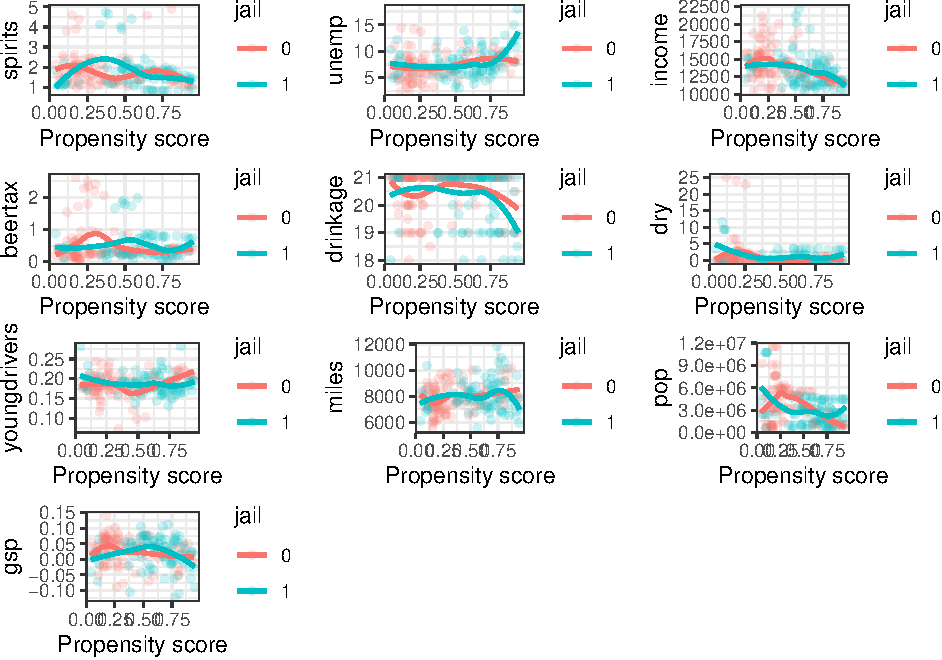
\includegraphics{Project3_Rongkui_files/figure-latex/unnamed-chunk-14-1.pdf}

\emph{Figure Y}: Propensity score distribution across two treatment
groups
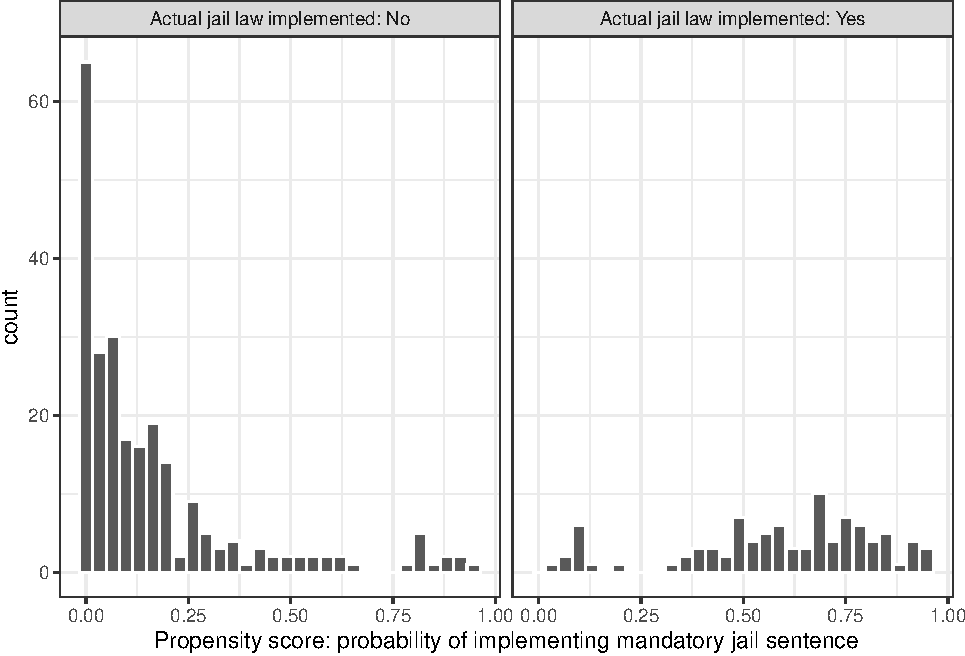
\includegraphics{Project3_Rongkui_files/figure-latex/unnamed-chunk-15-1.pdf}

\hypertarget{matching-1}{%
\subparagraph{3.2.2 Matching}\label{matching-1}}

Nearest neighbor matching algorithm resulted in a new dataset of 188
entires, with 94 original entries with mandatory jail sentence matched
with their respective non-treated entry with the most similar propensity
score.

\hypertarget{examining-covariate-balance-in-the-matched-sample-1}{%
\subparagraph{3.2.3 Examining covariate balance in the matched
sample}\label{examining-covariate-balance-in-the-matched-sample-1}}

\hypertarget{estimate-treatment-effect-1}{%
\subparagraph{3.2.4 Estimate Treatment
Effect}\label{estimate-treatment-effect-1}}

\hypertarget{model-diagnostics-1}{%
\paragraph{3.3 Model Diagnostics}\label{model-diagnostics-1}}

\hypertarget{goodness-of-fit-of-logistic-regression-model}{%
\subparagraph{3.3.1 Goodness-of-fit of logistic regression
model}\label{goodness-of-fit-of-logistic-regression-model}}

Unlike linear regression with ordinary least squares estimation, there
is no \(R^2\) statistic which explains the proportion of variance in the
dependent variable that is explained by the predictors. The most notable
pseudo \(R^2\) metric commonly used for assessing goodness-of-fit in
logistic regression is McFadden's \(R^2\), which is defined as
\(1−\frac{log(L_M)}{log(L_0)}\) where \(log(L_M)\) is the log likelihood
value for the fitted model and \(log(L_0)\) is the log likelihood for
the null model with only an intercept as a predictor. The
propensity-score-generating logistic regression model used in this study
has a McFadden's \(R^2\) of 0.39, indicating effective removal of a
large portion of confounded samples through the propensity score
matching process.

\hypertarget{mixed-effect-model}{%
\subparagraph{3.3.2 Mixed Effect model}\label{mixed-effect-model}}

The two crucial assumptions for a mixed effect model are normally
distributed residuals and constant variance of the residuals across the
fitted values, which will be discussed below. Influential observations
will also be discussed.

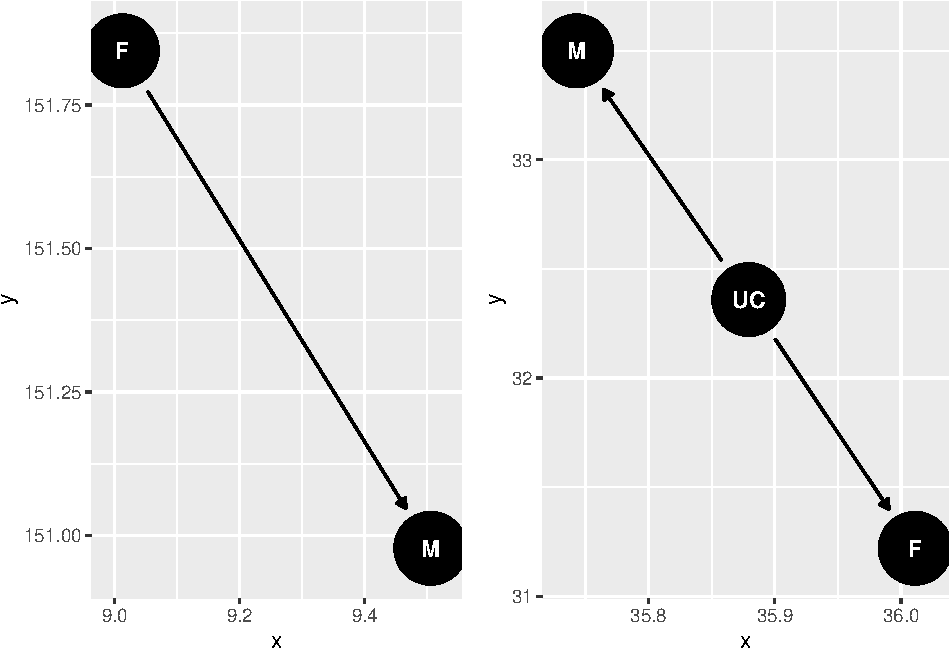
\includegraphics{Project3_Rongkui_files/figure-latex/unnamed-chunk-17-1.pdf}

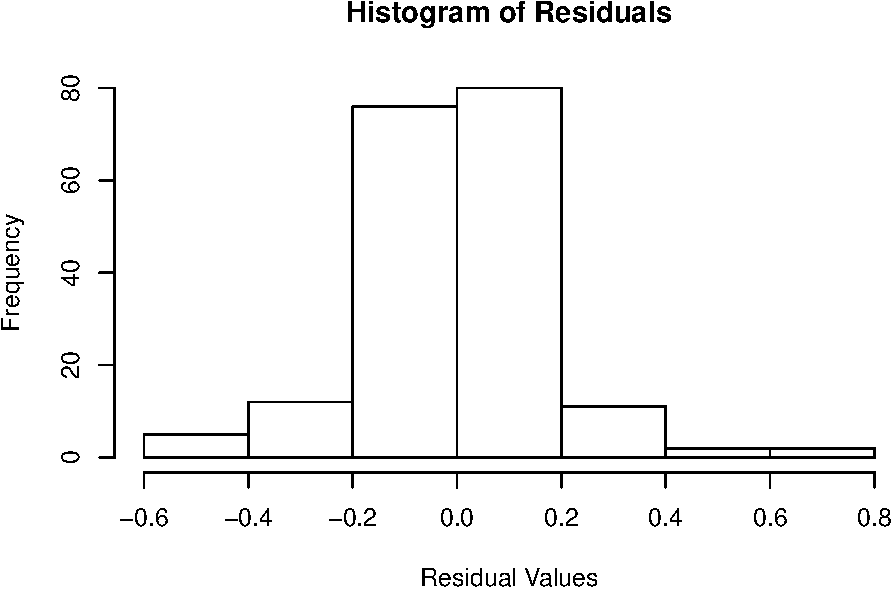
\includegraphics{Project3_Rongkui_files/figure-latex/unnamed-chunk-18-1.pdf}

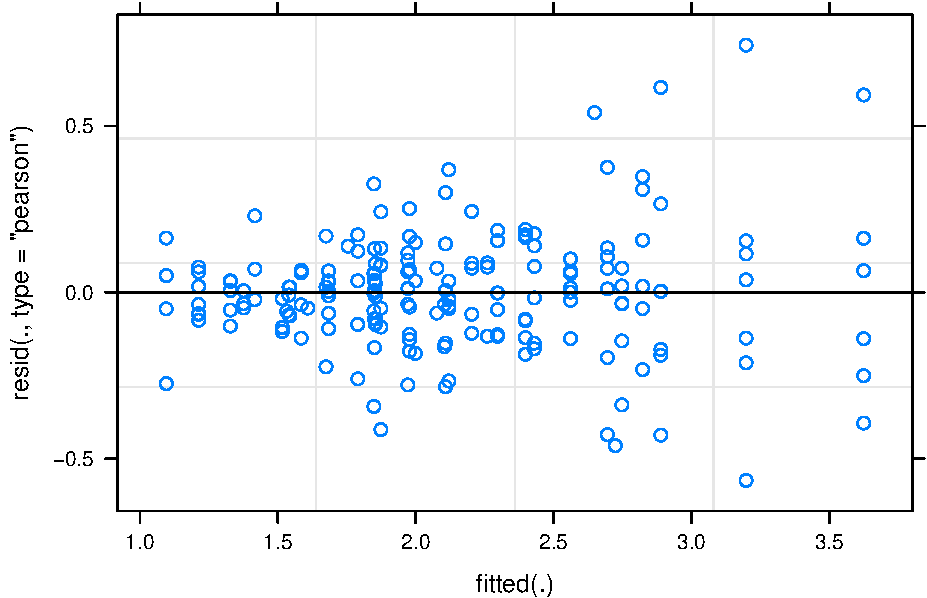
\includegraphics{Project3_Rongkui_files/figure-latex/unnamed-chunk-19-1.pdf}

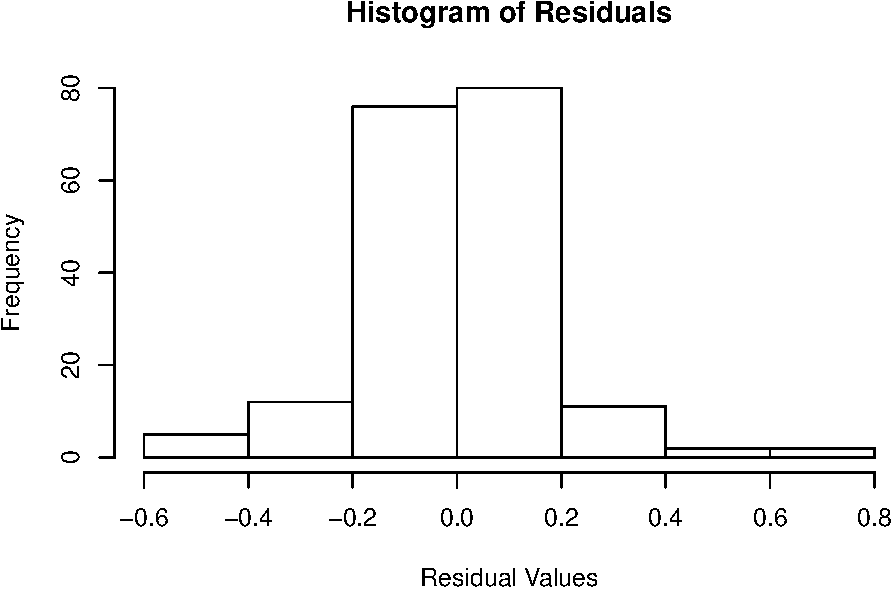
\includegraphics{Project3_Rongkui_files/figure-latex/unnamed-chunk-20-1.pdf}

Figure ..: Visual diagnostics of Mixed Effect model assumptions. (a).
Normal Q-Q plot of residuals. (b) Histogram of model residuals. (c)
Residuals-versus-fitted value scatter plot.

\hypertarget{normality}{%
\subparagraph{Normality:}\label{normality}}

From the Q-Q plot of the residuals (Figure ..a), we can see that the
probability mass on the left and right tails are higher than what is
expected from a normal distribution. The distribution of the residuals
seem to be heavy-tailed. Thus, the normality assumption is not satisfied
from the Q-Q plot. A histogram is used to visualize the distribution of
the residuals (Figure ..b). From the histogram, it is not easily
noticeable that the residuals do not follow a normal distribution.

To further test for normality of the errors, a Shapiro-Wilk test will be
used on the distribution of the residuals. A Shapiro-Wilk test is used
to test whether a distribution of data follows a normal distribution.

The null and alternative hypotheses of the Shapiro-Wilk test are:\\
\(H_0\): The residuals are normally distributed.\\
\(H_1\): The residuals are not normally distributed.

The p-value is essentially 0, and thus we reject the null hypothesis.
Thus, there is evidence that the distribution of the residuals do not
follow a normal distribution.

\hypertarget{equal-variances}{%
\subparagraph{Equal Variances:}\label{equal-variances}}

The spread of the residuals seem to increase along the x-axis in the
residuals-versus-fitted value scatter plot (Figure ..c), indicating
unequal variance of the residuals across the fitted values. Thus, the
equal variance assumption is not satisfied.

\hypertarget{influential-observations}{%
\paragraph{Influential Observations:}\label{influential-observations}}

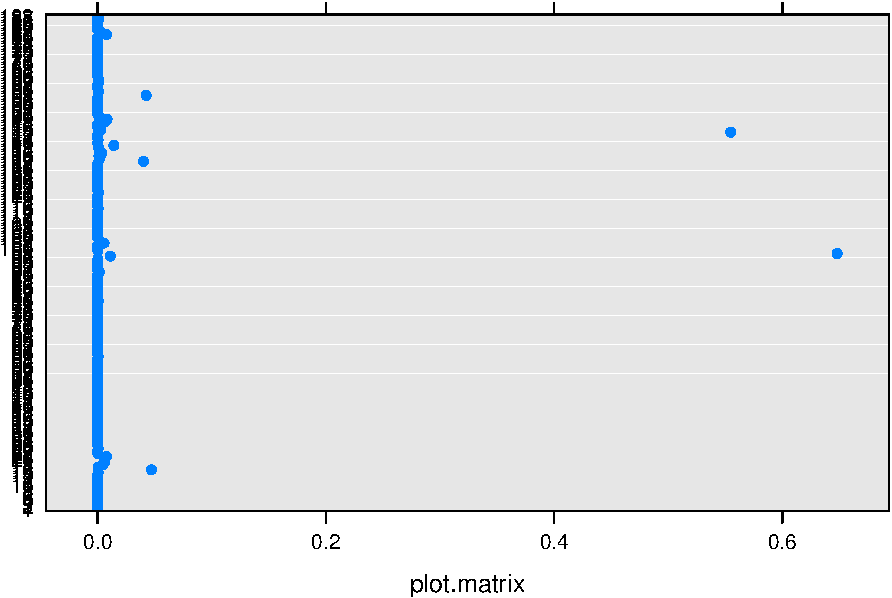
\includegraphics{Project3_Rongkui_files/figure-latex/unnamed-chunk-23-1.pdf}

Since the Cook's distance for every observation is less than 1, we
conclude that there are no highly influential observations.

\hypertarget{response-variable-transformation}{%
\subparagraph{Response Variable
Transformation:}\label{response-variable-transformation}}

In an attempt to remedy the departures of the assumptions of the mixed
effect model, we used a log transformation of the response variable, fr.
After the transformation, we concluded that the distribution of the
residuals did not follow a normal distribution after looking at a Normal
Q-Q plot and performing a Shapiro-Wilk test. The residuals did seem to
have more equal variance across the fitted values after the
transformation. Overall, a log transformation of the response variable
did not remedy the departures of the assumptions of the mixed effect
model.

\hypertarget{discussion}{%
\subsection{4.0 Discussion}\label{discussion}}

\hypertarget{propensity-score-matching}{%
\subsubsection{Propensity Score
Matching}\label{propensity-score-matching}}

In this report, we highlight the usage of propensity score matching for
isolating average treatment effect of implementing mandatory jail
sentence upon initial conviction of driving under influence. Rosenbaum
and Rubin (1983) defined treatment assignment to be strongly ignorable
if the following two conditions hold: (a) treatment assignment is
independent of the potential outcomes conditional on the observed
baseline covariates, and (b) every subject has a nonzero probability to
receive either treatment. They demonstrated that if treatment assignment
is strongly ignorable, conditioning on the propensity score allows one
to obtain unbiased estimates of average treatment effects. We achieved
these conditions through propensity score matching.

\hypertarget{causal-inference}{%
\subsubsection{Causal Inference}\label{causal-inference}}

We cannot confidently draw causal conclusions using the result from this
analysis. This is because of the violation of these assumptions
necessary for causal inference:

\begin{enumerate}
\def\labelenumi{\arabic{enumi}.}
\item
  The stable unit treatment value assumption (SUTVA):\\
  SUTVA states that the treatment assignment of one experimental unit
  cannot interfere with the outcome of a separate experimental unit.
  This is violated in this dataset because\\
\item
  temporal correlations across records taken from the same State, and
\item
  spacial correlations among states that are geographically close to
  each other.\\
  The implementation of mandatory jail sentence in one state is very
  likely to influence the vehicle fatality of an adjacent state. And the
  historic state of the legislation is very likely to influence the
  vehicle fatality of the same state in the years to come.
\item
  Exogeneity: The exogeneity assumption states that the independent
  variable (implementation of mandatory jail sentence) cannot be
  dependent on the dependent variable (vehicle fatality rate). This
  assumption is likely to be violated in this dataset because
  legislations can arise from existing conditions (\emph{Figure Za}).
\item
  Ignorabilty of unobserved potential confounding variables: Although
  this expansive dataset captures many prominent variables that are
  associated with vehicle fatality rate, many more economic and social
  factors come into play in impacting the interactions between the
  implementation of mandatory jail sentence and vehicle fatality rate.
  We cannot confidently exclude the possiblity of the existence of many
  of such variables (\emph{Figure Zb}).
\end{enumerate}

Ultimately, our analysis makes very improbable assumptions in order to
analyze this observational data. Due to this lack of strong assumptions
around SUTVA and observation of all covariates, we fail to make any
strong causal conclusions regarding the effect of mandatory jail
sentences on State fatality rates.

Due to this lack of clear causality, we propose State legislators focus
their energy and capital on measures directly correlated with the
probability of entering a fatal collision. Better seatbelt enforcement,
speeding enforcement, and drunk driver intervention have all
demonstrated their effectiveness at better-protecting citizens and
reducing the risk of a fatal accident (Morley, 2016). Legislators should
focus on active measures to combat fatal automobile collisions instead
of hoping to find a strong causal effect in passive measures like
mandatory jail sentencing.

\hypertarget{reference}{%
\subsection{5.0 Reference}\label{reference}}

Austin P. C. (2011). An Introduction to Propensity Score Methods for
Reducing the Effects of Confounding in Observational Studies.
Multivariate behavioral research, 46(3), 399--424.
\url{doi:10.1080/00273171.2011.568786}

Brookhart M.A., Schneeweiss S., Rothman K.J., Glynn R.J., Avorn J.,
Stürmer T. (2006). Variable selection for propensity score models.
American Journal of Epidemiology. 163, 1149--1156.\\
Rosenbaum P.R., Rubin D.B. (1983). The central role of the propensity
score in observational studies for causal effects. Biometrika.
70:41--55.

Durbin, D. R., Elliott, M. R., \& Winston, F. K. (2009). A propensity
score approach to estimating child restraint effectiveness in preventing
mortality. Statistics and Its Interface, 2(4), 437--447. doi:
10.4310/sii.2009.v2.n4.a5

Morley, A., Morris, A., Abi Semaan, M., \& Hancox, G. (2016). A Guide
for Policy Makers: On Reducing Road Fatalities. Retrieved from
\url{https://www.pwc.com/m1/en/publications/guide-on-reducing-road-fatalities.html}

Rodriguez, D., Rejesus, R., \& Aragon, C. (2007). Impacts of an
Agricultural Development Program for Poor Coconut Producers in the
Philippines: An Approach Using Panel Data and Propensity Score Matching
Techniques. Journal of Agricultural and Resource Economics, 32(3),
534-557. Retrieved February 14, 2020, from www.jstor.org/stable/40982695

Rosenbaum, P., \& Rubin, D. (1983). The Central Role of the Propensity
Score in Observational Studies for Causal Effects. Biometrika, 70(1),
41-55. \url{doi:10.2307/2335942}

Sasidharan, L., \& Donnell, E. T. (2013). Application of propensity
scores and potential outcomes to estimate effectiveness of traffic
safety countermeasures: Exploratory analysis using intersection lighting
data. Accident Analysis \& Prevention, 50, 539--553. doi:
10.1016/j.aap.2012.05.036

Smith, H. L. (1997). 6. Matching with Multiple Controls to Estimate
Treatment Effects in Observational Studies. Sociological methodology,
27(1), 325-353.

\end{document}
